\documentclass[11pt]{article}
\usepackage[a4paper,margin=22mm]{geometry}
\usepackage{amsmath,amssymb,booktabs,longtable,array,enumitem,graphicx,xcolor}
\usepackage[hidelinks]{hyperref}
\usepackage{tikz}
\usetikzlibrary{arrows.meta,positioning,calc,shapes.geometric}
\setlength{\parindent}{0pt}
\setlength{\parskip}{6pt}
\setlist[itemize]{nosep}
\setlist[enumerate]{itemsep=3pt}
\newcommand{\sol}{\paragraph{Solution.}}
\newcommand{\SA}{\mathrm{SA}}
\newcommand{\up}{\mathord{\Uparrow}}
\newcommand{\dn}{\mathord{\Downarrow}}
\newcommand{\any}{\mathord{\Updownarrow}}
\hypersetup{pdftitle={VLSI Testing: rebuilt examination and independent solutions},pdfauthor={}}
\begin{document}
\title{VLSI Testing: 2014 Midterm}\author{}\date{}\maketitle\begin{quote}\small
Reconstructed questions and independently derived solutions. Personal names, identifiers,
handwritten answers and administrative headers are omitted. Figures are redrawn as
logical diagrams or explicit netlists. A source-reading note identifies a meaningful
ambiguity instead of silently changing the question. Finite Boolean checks
are supplied in the examination collection's Python verification script.
\end{quote}

\section{Single-cell faults in a ripple-carry adder}
\textbf{Question.} An $n$-bit ripple-carry adder is built from full-adder cells.
Derive a test set covering every single cell fault with a size independent of $n$.
The cell outputs are sum and carry.
\begin{center}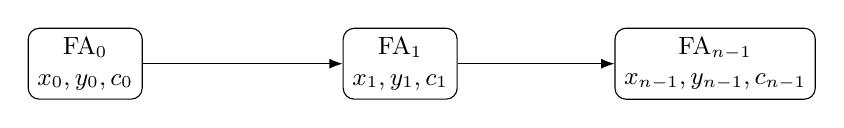
\begin{tikzpicture}[>=Latex,box/.style={draw,rounded corners,align=center,minimum height=9mm,font=\small},scale=1,transform shape]
\node[box] (fa1) at (0,0) {FA$_0$\\$x_0,y_0,c_0$};
\node[box] (fa2) at (4,0) {FA$_1$\\$x_1,y_1,c_1$};
\node[box] (fan) at (8,0) {FA$_{n-1}$\\$x_{n-1},y_{n-1},c_{n-1}$};
\draw[->] (fa1) -- (fa2);
\draw[->] (fa2) -- (fan);
\end{tikzpicture}\end{center}

\sol A single faulty cell may implement any incorrect truth table, so apply all
eight $(x_i,y_i,c_i)$ triples to every cell. Use the following eight whole-adder tests:
\begin{enumerate}
\item Four tests: every bit has $(x_i,y_i)=01$, with $c_0=0$ and $1$;
then every bit has $(x_i,y_i)=10$, again with $c_0=0$ and $1$.
Both pairs propagate carry, so every cell sees the selected carry.
\item One test: all pairs are $00$ and $c_0=0$.
One test: all pairs are $11$ and $c_0=1$.
\item One test alternates $00,11,00,11,\ldots$ from the least significant cell,
with $c_0=1$. The other alternates $11,00,11,00,\ldots$, with $c_0=0$.
Thus every cell sees both $001$ and $110$ across these two tests.
\end{enumerate}
The eight local triples are now covered at every position. A wrong sum is directly
observable. A wrong carry changes the next good cell's sum (sum is XOR in carry);
at the last cell it is the primary carry output. Therefore one faulty cell cannot
hide its error under this model. The number of tests is eight, independent of $n$.
This argument assumes all sum bits and the final carry are observed and only one
cell is faulty.
\section{ATPG by the D-algorithm and single-path sensitization}
\textbf{Question.} Generate a test for $x/0$ using the D-algorithm and a test
for $y/0$ using single-path sensitization, for the following circuit.
\begin{center}\begin{tabular}{ll}\toprule Signal & Defining expression\\\midrule
$u$ & $\overline{C+D}$\\
$g$ & $Bu$\\
$h$ & $\overline{A+g}$\\
$i$ & $gE$\\
$F$ & $h+i$\\
\bottomrule\end{tabular}\end{center}
\begin{center}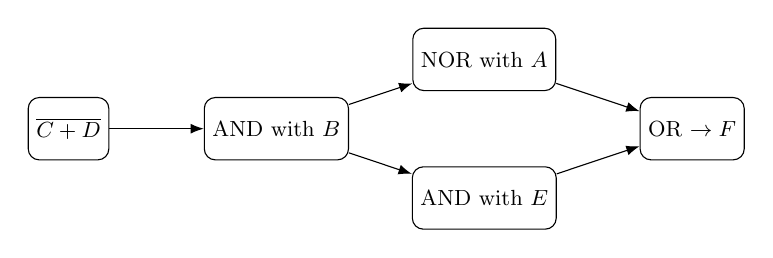
\begin{tikzpicture}[>=Latex,box/.style={draw,rounded corners,align=center,minimum height=9mm,font=\small},scale=0.88,transform shape]
\node[box] (u) at (0,0) {$\overline{C+D}$};
\node[box] (g) at (3,0) {AND with $B$};
\node[box] (h) at (6,1) {NOR with $A$};
\node[box] (i) at (6,-1) {AND with $E$};
\node[box] (f) at (9,0) {OR $\to F$};
\draw[->] (u) -- (g);
\draw[->] (g) -- (h);
\draw[->] (g) -- (i);
\draw[->] (h) -- (f);
\draw[->] (i) -- (f);
\end{tikzpicture}\end{center}
\sol The scan marks $y/0$ on $B$ and $x/0$ near the lower fanout
branch of $g$. For $x/0$, choose $(A,B,C,D,E)=11001$:
$u=g=E=1$, $h=0$, and the lower AND carries $D=(1,0)$ to $F$.
This vector detects both a lower-branch fault and a whole-stem $g/0$ fault.
For $y/0$ on $B$, use $01000$: $u=1$, the good/faulty $g$ is $D$,
$A=0$ sensitizes the upper NOR and $E=0$ blocks the lower branch.
Thus $F=\bar D$.\section{Combinational SCOAP}
\textbf{Question.} Compute controllability and observability for every signal in the following netlist.

Use $CC_0=CC_1=1$ at a primary input and $CO=0$ at a primary output;
each gate adds one. For an AND gate,
$CC_0=1+\min CC_0(i)$ and $CC_1=1+\sum CC_1(i)$.
For an OR gate, interchange the roles of 0 and 1.
NAND/NOR swap the two output controllabilities; an inverter swaps its input
values and adds one. To observe one gate input, set the other inputs to their
noncontrolling values, add their controllability costs, add $CO$ of the output
and add one. At a fanout stem take the minimum branch $CO$.
For XOR/XNOR, minimize the sum of input costs subject to the desired parity.
These are structural SCOAP estimates; reconvergent inputs are treated independently.
\begin{center}\begin{tabular}{ll}\toprule Signal & Defining expression\\\midrule
$N$ & $X_2X_3$\\
$J$ & $\bar X_4$\\
$I$ & $\bar X_3$\\
$E$ & $X_1N$\\
$M$ & $NJ$\\
$L$ & $IX_4$\\
$F$ & $E+M+L$\\
\bottomrule\end{tabular}\end{center}
Here $F$ is the only primary output.
Handwritten numbers in the source are not an answer key.
\begin{center}\begin{tabular}{lrrr}\toprule
Signal & $CC_0$ & $CC_1$ & $CO$\\\midrule
$X1$ & 1 & 1 & 10\\
$X2$ & 1 & 1 & 10\\
$X3$ & 1 & 1 & 9\\
$X4$ & 1 & 1 & 9\\
$N$ & 2 & 3 & 8\\
$J$ & 2 & 2 & 9\\
$I$ & 2 & 2 & 8\\
$E$ & 2 & 5 & 6\\
$M$ & 3 & 6 & 5\\
$L$ & 2 & 4 & 6\\
$F$ & 8 & 5 & 0\\
\bottomrule\end{tabular}\end{center}
For example,
$CC_0(F)=2+3+2+1=8$ and $CC_1(F)=1+\min(5,6,4)=5$.
Branch $CO$ values are $N\to E=8$, $N\to M=8$,
$X_3\to N=10$, $X_3\to I=9$,
$X_4\to J=10$, $X_4\to L=9$.
\section{Deductive fault simulation}
\textbf{Question.} The circuit is
$N=\overline{D+E}$, $P=AB$, $Q=CG$, $R=FH$, $Z=P+Q+R$,
where $G$ and $H$ are separate branches of $N$.
The four faults are $f_A=A/1$, $f_E=E/0$, $f_G=G/1$, $f_H=H/1$.
Find detected faults for $(A,B,C,D,E,F)=011011$ and $011111$.
\begin{center}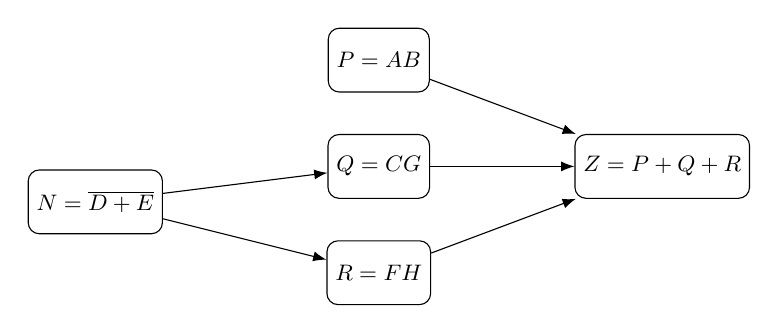
\begin{tikzpicture}[>=Latex,box/.style={draw,rounded corners,align=center,minimum height=9mm,font=\small},scale=0.9,transform shape]
\node[box] (n) at (0,-1) {$N=\overline{D+E}$};
\node[box] (p) at (4,1) {$P=AB$};
\node[box] (q) at (4,-0.5) {$Q=CG$};
\node[box] (r) at (4,-2) {$R=FH$};
\node[box] (z) at (8,-0.5) {$Z=P+Q+R$};
\draw[->] (n) -- (q);
\draw[->] (n) -- (r);
\draw[->] (p) -- (z);
\draw[->] (q) -- (z);
\draw[->] (r) -- (z);
\end{tikzpicture}\end{center}

\sol Both patterns have $(P,Q,R)=(0,0,0)$ and $Z=0$.
For $011011$, $D=0,E=1$, so $E/0$ changes $N$ from 0 to 1.
Deductive lists are
\[
L(P)=\{f_A\},\quad L(N)=\{f_E\},\quad
L(Q)=\{f_E,f_G\},\quad L(R)=\{f_E,f_H\}.
\]
All OR inputs are zero, so take the union:
$L(Z)=\{f_A,f_E,f_G,f_H\}$.
For $011111$, $D=1$ masks $E/0$ at the NOR gate.
Consequently $L(N)=\varnothing$, $L(Q)=\{f_G\}$,
$L(R)=\{f_H\}$ and $L(Z)=\{f_A,f_G,f_H\}$.
The branches $G,H$ must be kept distinct; a stem fault is a different fault.
\section{Fault tests for a mux network}
\textbf{Question.} Find two tests for the marked SA0 and SA1 faults.
\begin{center}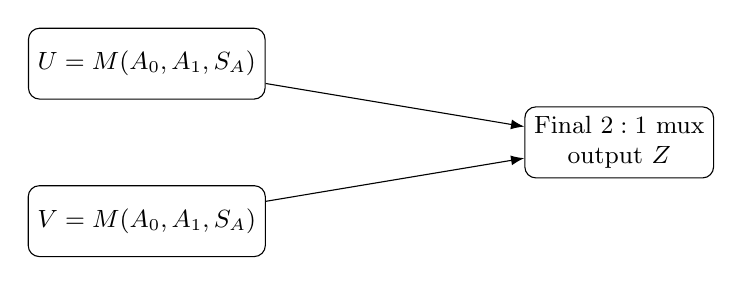
\begin{tikzpicture}[>=Latex,box/.style={draw,rounded corners,align=center,minimum height=9mm,font=\small},scale=1,transform shape]
\node[box] (u) at (0,1) {$U=M(A_0,A_1,S_A)$};
\node[box] (vv) at (0,-1) {$V=M(A_0,A_1,S_A)$};
\node[box] (z) at (6,0) {Final $2:1$ mux\\output $Z$};
\draw[->] (u) -- (z);
\draw[->] (vv) -- (z);
\end{tikzpicture}\end{center}
\sol Let $U=M(A_0,A_1,S_A)$, $V=M(A_0,A_1,S_A)$ and
$Z=M(U,V,S)$, with $M(a,b,s)=\bar s a+sb$.
The faults are $U/0$ and the lower mux's $S_A$ branch stuck at 1.
For $U/0$, use $(A_0,A_1,S_A,S)=1000$, giving $Z=1/0$.
For the lower-select fault, use $0101$: the lower mux is selected,
its good data is $A_0=0$ and its faulty data is $A_1=1$.
Thus $Z=0/1$. Keep the lower-select branch distinct from the common stem.
\section{Short questions on manufacturing test}
\begin{enumerate}[label=(\alph*)]
\item \textbf{Verification and test.} Verification asks whether the design implements
the specification. Manufacturing test applies stimuli to fabricated hardware and
checks for physical defects represented by a fault model.
\item \textbf{Yield and defect level.} With yield $Y=0.5$, use the model
$DL=1-Y^{1-FC}$ for the defect fraction among shipped parts.
For $DL\le100\times10^{-6}$,
\[
 FC\ge1-\frac{\ln(0.9999)}{\ln(0.5)}
 =0.99985572\ldots,
\]
so at least $99.9856\%$ fault coverage is required \emph{under this model}.
Yield alone cannot determine defect level without a coverage/escape model.
\item \textbf{Test flow.} Select a defect/fault model; generate and simulate tests;
prepare tester programs and expected responses; apply tests at wafer/package/board
stages as appropriate; compare responses, diagnose failures and bin devices;
feed results back to design and manufacturing.
\item \textbf{Detection, location, diagnosis.} Detection distinguishes faulty from
fault-free behavior. Location narrows the physical or logical site. Diagnosis
infers likely fault mechanisms/sites from the response syndrome.
\item \textbf{Fault modeling.} A finite logical/electrical abstraction of defects makes
test generation and coverage measurable; model coverage need not equal defect coverage.
\item \textbf{Bathtub curve.} Early failures decrease as weak parts fail;
useful life has a low approximately constant hazard;
wear-out failures increase with aging.
\item \textbf{Fault coverage.} $FC=N_{\rm detected}/N_{\rm modeled}$, with the
denominator and any exclusion of untestable faults stated explicitly.
\item \textbf{Fault simulation.} Predict faulty responses, measure coverage, identify
undetected faults and grade/compact tests; optionally provide diagnostic signatures.
\end{enumerate}
\begin{center}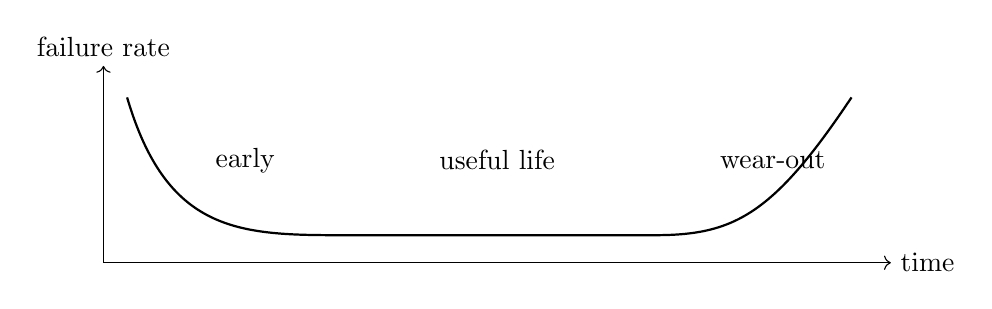
\begin{tikzpicture}[x=1cm,y=1cm]
\draw[->](0,0)--(10,0) node[right]{time};
\draw[->](0,0)--(0,2.5) node[above]{failure rate};
\draw[thick] (0.3,2.1) .. controls (.8,.4) and (1.7,.35) .. (3,.35)
 --(7,.35) .. controls(8,.35) and(8.5,.6) ..(9.5,2.1);
\node at(1.8,1.3){early};\node at(5,1.3){useful life};\node at(8.5,1.3){wear-out};
\end{tikzpicture}\end{center}

\section{Equivalence and dominance}
\textbf{Question.} For $d=\overline{ab}$ and $e=\overline{d+c}$, classify
$a/0$, $b/1$, $d/1$ and $e/0$ by equivalence and dominance.
\begin{center}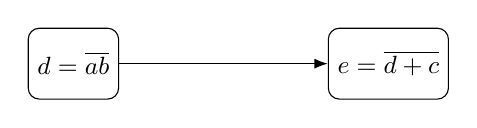
\begin{tikzpicture}[>=Latex,box/.style={draw,rounded corners,align=center,minimum height=9mm,font=\small},scale=1,transform shape]
\node[box] (d) at (0,0) {$d=\overline{ab}$};
\node[box] (e) at (4,0) {$e=\overline{d+c}$};
\draw[->] (d) -- (e);
\end{tikzpicture}\end{center}

\sol Since $e=ab\bar c$, the detection sets, in $(a,b,c)$ order, are
\[
T(a/0)=T(d/1)=T(e/0)=\{110\},\qquad T(b/1)=\{100\}.
\]
Thus the first three faults are equivalent. The fourth is neither equivalent to
nor in a strict dominance relationship with them: the two nonempty detection
sets are disjoint. Stating the sets also avoids opposite conventions for dominance.

\end{document}
